%!TEX program = xelatex
\documentclass{article}
\textwidth 150mm \textheight 220mm \oddsidemargin 5mm
\evensidemargin 5mm \topmargin -10mm
\usepackage{amsmath}
\usepackage{amsfonts,amssymb}
\usepackage{fontspec}
\usepackage{microtype}
\usepackage{setspace}
\usepackage{multirow}
\usepackage{blkarray}
\usepackage{tikz}
\usepackage{dsfont}
\usepackage{booktabs}
\usepackage{enumerate}
%\usepackage{indentfirst}
\usepackage{mathrsfs}
\usepackage{listings}
%\usepackage[usenames,dvipsnames]{xcolor}
\usepackage{epsf}
\usepackage[linesnumbered,boxed]{algorithm2e}
\usepackage[colorlinks,linkcolor=red]{hyperref}
\renewcommand\thesection{\Roman{section}}%\arabic{section}}
\renewcommand\thesubsection{\Roman{section.}\roman{subsection})}
\renewcommand\thesubsubsection{\arabic{subsubsection}.}
\defaultfontfeatures{Mapping=tex-text,Scale=MatchLowercase}
%\setmainfont{Citadel Script}
\setmainfont{Savoye LET}
%\setmainfont{Chalkboard}
%\setmainfont{Optima}
%\setmainfont{Apple Chancery}
\setmonofont{Optima}
\setsansfont{Optima}
%\renewcommand{\familydefault}{\sfdefault}
%\renewcommand{\footnotesize}{\sfdefault}
\setlength{\parskip}{\baselineskip}
\setlength{\parindent}{0em}
%%%%%%%%%%%Here is the configurations for Code%%%%%%%%%%%

\definecolor{mygreen}{rgb}{0,0.6,0}
\definecolor{mygray}{rgb}{0.5,0.5,0.5}
\definecolor{mymauve}{rgb}{0.58,0,0.82}
\lstset{
 backgroundcolor=\color{white}, 
 basicstyle = \footnotesize,       
 breakatwhitespace = false,        
 breaklines = true,                 
 captionpos = b,                    
 commentstyle = \color{mygreen}\bfseries,
 extendedchars = false,             
 frame =shadowbox, 
 framerule=0.5pt,
 keepspaces=true,
 keywordstyle=\color{blue}\bfseries, % keyword style
 language = C++,                     % the language of code
 otherkeywords={string}, 
 numbers=left, 
 numbersep=5pt,
 numberstyle=\tiny\color{mygray},
 rulecolor=\color{black},         
 showspaces=false,  
 showstringspaces=false, 
 showtabs=false,    
 stepnumber=0,         
 stringstyle=\color{mymauve},        % string literal style
 tabsize=2,          
 title=\lstname                      
}

%%%%%%%%%%%%%%%%%%%%%%%%%%%%%%%%%%%%%%%%%%%%

\begin{document}
\renewcommand\arraystretch{1.5}


\thispagestyle{empty}

\begin{center}
\begin{large}
\begin{figure}[!htbp]
\centering

\includegraphics[width=0.7\textwidth]{Logo2.png}
\end{figure}
\hrule
\vspace*{0.25cm}
\sc{UM--SJTU Joint Institute \vspace*{0.3em}} \\ 
VE281 Project 1\\
\end{large}
\hrulefill

\vspace*{5cm}

\begin{Large}
\sc{{Report}} \\
\end{Large}
\vspace*{2em}
\begin{large}
\sc{{Tianze Wang, 515370910202}}
\end{large}
\end{center}
\newpage
\setmainfont{Optima}
\setcounter{page}{1}
\section{Introduction}
\par We've written six sorting algorithms in Project 1. And we will compare their performances in this report.
\section{Methods Used}
\par To compare them, we first need an algorithm to generate random numbers. The code is shown as below.
	\begin{lstlisting}[caption={}]
#include <iostream>
#include <fstream>
#include <sstream>
#include <string>
#include <cstdlib>
#include <climits>
#include <ctime>
#include <random>

using namespace std;

int main(int argc, char * argv[]) {
    int n = atoi(argv[1]);
    int m = atoi(argv[2]);
    cout << n << endl;
    cout << m << endl;
    srand((unsigned) time(NULL));
    for (int i=0;i<m;i++){
        cout << mrand48() << endl;
    }
}
\end{lstlisting}
This code above is used to generate array of integers ranging in $\left[ -2^{31}, 2^{31}-1\right]$, and we name the program as ``generator''. To generate the code with less efforts, we need a function to generate bunch of instructions simultaneously.
\begin{lstlisting}
#include <iostream>
#include <random>

using namespace std;

int main(int argc, char * argv[]) {
    int n = atoi(argv[1]);
    int m = atoi(argv[2]);

    for (int i = 0; i<=5; i++) {
        for (int j=5; j <= 50000; j*=10)
        cout << "./generator " << i << " " << j << " > " << "Test_" << i << "_" << j<< endl;
    }
}
\end{lstlisting}
And we run the result in the directory of generator, to get $5 \cdot 6=30$ groups of inputs, with 5 categories, namely \[
	5,50,500,5000,50000
\]
increasing in 10 times, to test the performance of each algorithm.
\par And we run it in bash, with the result generated by
\begin{lstlisting}
#include <iostream>
#include <fstream>
#include <sstream>
#include <string>
#include <cstdlib>
#include <climits>
#include <ctime>
#include <random>

using namespace std;

int main(int argc, char * argv[]) {
    int n = atoi(argv[1]);
    int m = atoi(argv[2]);

    for (int i = 0; i<=5; i++) {
        for (int j=5; j <= 50000; j*=10)
        cout << "./p3 "<< "< Test_" << i << "_" << j<< endl;
    }
}
\end{lstlisting}
And the test result is shown as below. Here I slightly changed the main function of project to make it only output the runtime of each function. \newpage
\section{A table comparing 6 sort methods}
\begin{table}[!htbp]
  \centering
    \begin{tabular}{|c|ccccc|} \hline
   Sort name(in seconds) $\backslash$  Test number & 5     & 50    & 500   & 5000  & 50000 \\ \hline
    Bubble & 2.00E-06 & 1.30E-05 & 0.001163 & 0.08668 & 11.81 \\  
    Insertion & 1.00E-06 & 5.00E-06 & 0.000274 & 0.020239 & 2.27562 \\  
    Selection & 2.00E-06 & 7.00E-06 & 0.000607 & 0.040228 & 3.72899 \\ 
    Merge & 3.00E-06 & 1.20E-05 & 0.000139 & 0.001594 & 0.033226 \\  
    Quick ExtraArray & 1.20E-05 & 2.10E-05 & 0.000196 & 0.001336 & 0.015471 \\
    Quick Inplace & 2.00E-06 & 4.00E-06 & 8.40E-05 & 0.000657 & 0.010704 \\ \hline
    \end{tabular}%
    \caption{The comparison result.}
\end{table}%
We found the scale is not easy to be shown a linear axis, so we take logarithm of all values. And we will then get the following table.
\begin{table}[!htbp]
  \centering
    \begin{tabular}{|c|ccccc|} \hline
   Sort name(in seconds) $\backslash$  Test number & 0.69897 & 1.69897 & 2.69897 & 3.69897 & 4.69897 \\ \hline
    Bubble & -5.69897 & -4.886057 & -2.93442 & -1.062081 & 1.0722499 \\
    Insertion & -6    & -5.30103 & -3.562249 & -1.693811 & 0.3570997 \\
    Selection & -5.69897 & -5.154902 & -3.216811 & -1.395472 & 0.5715912 \\
    Merge & -5.522879 & -4.920819 & -3.856985 & -2.797512 & -1.478522 \\
    Quick ExtraArray & -4.920819 & -4.677781 & -3.707744 & -2.874194 & -1.810482 \\
    Quick Inplace & -5.69897 & -5.39794 & -4.075721 & -3.182435 & -1.970454 \\ \hline 
        \end{tabular}%
    \caption{The comparison result in logarithm unit.}
\end{table}%
\begin{flushleft}
And to make it clearer, we draw a plot with six curves showing different result of the second graph.
\end{flushleft}

\begin{figure}[t]
\centering
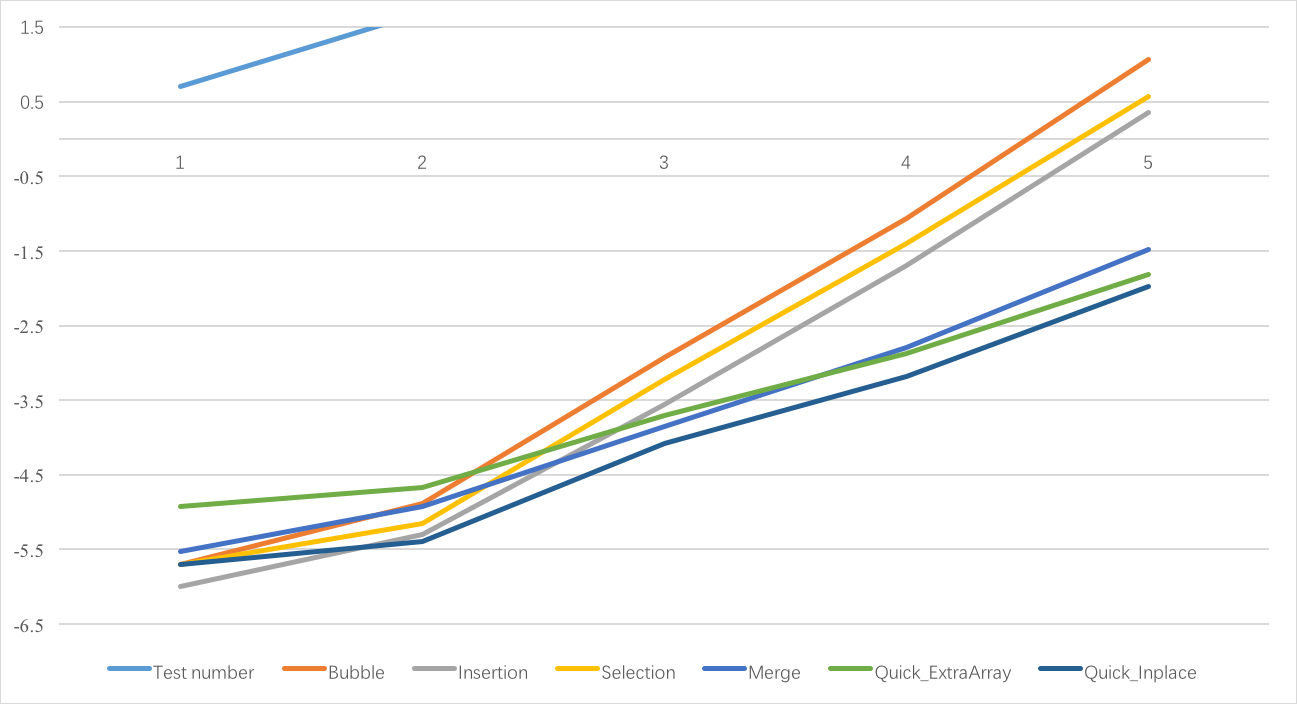
\includegraphics[width=\textwidth]{pic1.png}
\caption{Comparison result in Logarithm}
\end{figure}
\newpage
\section{Discussion and Conclusion}
From the graph, it's easy to conclude three points:
\begin{itemize}
\item For small arrays (less than 500 items), bubble, insertion and selection sort has better performance than merge sort and quick sort.
\item For large arrays (More than 500 items), merge sort and quick sort perform better.
\item For the two quick sorts, in-place performs better than using an extra array.
\end{itemize}
So we can conclude that for larger array, we'd better use in-place quick sort and merge sort. 
\section{Appendix}
Please see the source code in this part.
\begin{lstlisting}
#include <iostream>
#include <fstream>
#include <sstream>
#include <string>
#include <cstdlib>
#include <climits>
#include <ctime>
#include "sort.h"

using namespace std;

int main() {
    int sort_num, len;
    double dur;
    clock_t start,end;
    cin >> sort_num;
    cin >> len;
    int *arr = new int[len];
    int i;
    for (i = 0; i < len; i++) {
        cin >> arr[i];
    }
    start= clock();
    if (sort_num == 0) {
        bubble(arr, len);
    } else if (sort_num == 1) insertion(arr, len);
    else if (sort_num == 2) selection(arr, len);
    else if (sort_num == 3) merge(arr, 0, len - 1, len);
    else if (sort_num == 4) quick_extra(arr, len);
    else if (sort_num == 5) quick_inPlace(arr, 0, len - 1);
    end = clock();

//    for (i = 0; i < len; i++) {
//        cout << arr[i] << endl;
//    }
    dur= (double) end-start;
    cout << dur/CLOCKS_PER_SEC<< endl;
//    cout << len;

    delete[] arr;
    return 0;
}

void bubble(int arr[], int length) {
    int i, j;
    for (i = 0; i < length; i++) {
        for (j = 0; j < length - i - 1; j++) {
            if (arr[j] > arr[j + 1]) {
                swap(arr[j], arr[j + 1]);
            }
        }
    }
}

void insertion(int arr[], int length) {
    int i, j;
    for (i = 1; i < length; i++) {
        auto temp = arr[i];
        j = i - 1;
        while (j >= 0 && arr[j] > temp) {
            arr[j + 1] = arr[j];
            j--;
        }
        arr[j + 1] = temp;
    }
}

void selection(int arr[], int length) {
    int i, j, temp, temp_id;
    for (i = 0; i < length - 1; i++) {
        temp = arr[i];
        temp_id = i;
        for (j = i + 1; j < length; j++) {
            if (arr[j] < temp) {
                temp = arr[j];
                temp_id = j;
            }
        }
        swap(arr[i], arr[temp_id]);
    }
}


//void merge_sort(int arr[], int left, int mid, int right) {
//    int i = 0, j = 0, k = 0;
//    //int arr2[right - left + 1];
//    auto *arr2 = new int[right-left+1];
//    while (i < mid - left + 1 && j < right - mid) {
//        if (arr[i] <= arr[j + mid]) arr2[k++] = arr[i++];
//        else arr2[k++] = arr[mid + (j++)];
//    }
//    if (i == mid - left) {
//        while (k < right) {
//            arr2[k] = arr[mid + j];
//            k++;
//            j++;
//        }
//    } else {
//        while (k < right) {
//            arr2[k] = arr[mid + i];
//            i++;
//            k++;
//        }
//    }
//    delete[] arr2;
//}


void merge_sort(int arr[], int left, int mid, int right, int len) {
    auto arr2 = new int[len];

    int i;

    i = left;
    int j = mid + 1, k = left;

    while (i <= mid && j <= right) {
        if (arr[i] <= arr[j]) {
            arr2[k++] = arr[i++];
        } else {
            arr2[k++] = arr[j++];
        }
    }
    int j1;
    if (i > mid) {
        for (j1 = j; j1 <= right; j1++) {
            arr2[k++] = arr[j1];
        }
    } else {
        for (j1 = i; j1 <= mid; j1++) {
            arr2[k++] = arr[j1];
        }
    }

    for (i = left; i <= right; i++) {
        arr[i] = arr2[i];
    }
    delete[] arr2;
}


void merge(int arr[], int left, int right, int len) {
    if (left >= right) return;
    int mid = (left + right) / 2;
    merge(arr, left, mid, len);
    merge(arr, mid + 1, right, len);
    merge_sort(arr, left, mid, right, len);
}

//Partition with external array

int partition_ex(int arr[], int len) {
    int rand1= rand()% len;
    swap(arr[0],arr[rand1]);
    int i = 0;
    int k = 0;
    int j = len -1;
    auto arr2 = new int[len];

    for (i = 1; i < len; i++) {
        if (arr[i] < arr[0]) {
            arr2[k++] = arr[i];
        } else arr2[j--] = arr[i];
    }
    arr2[k] = arr[0];
    for (i = 0; i < len; i++) {
        arr[i] = arr2[i];
    }
    delete[] arr2;
    return k;
}

//Partition in place

// int partition_ip(int *arr, int left, int right) { // referred to page 4 of slide 6
//     int pivot_chosen = (rand() % (right - left + 1)) + left;
//     int len = right - left + 1;
//     int i = left + 1;
//     int j = right;
//     while (1) {
//         while (arr[i] < arr[pivot_chosen] && i < right) { i++; }
//         while (arr[j] >= arr[pivot_chosen] && j > left) { j--; }
//         if (i < j) { swap(arr[i], arr[j]); }
//         else break;
//     }
//     swap(arr[left], arr[j]);
//     return j;
// }
//int partition_ip(int arr[], int left, int right) { // referred to page 4 of slide 6
////    int pivot_chosen = (rand() % (right - left + 1)) + left;
//    int len = right - left + 1;
//    int i = left + 1;
//    int j = right-1;
////    swap(arr[pivot_chosen],arr[left]);
//    while (1) {
//        while (arr[i] < arr[left] && i < right) { i++; }
//        while (arr[j] >= arr[left] && j > left) { j--; }
//        if (i < j) { swap(arr[i], arr[j]); }
//        else break;
//    }
//    swap(arr[left], arr[j]);
//    return j;
//}

//void quick_extra(int arr[], int left, int right) {
//    int pivotat;
//    if (left >= right) {
//        return;
//    }
//    pivotat = partition_ex(arr, left, right);
//    swap(arr[left], arr[pivotat]);
//    quick_extra(arr, left, pivotat - 1);
//    quick_extra(arr+pivotat+1, pivotat + 1, right);
//}
void quick_extra(int arr[], int len) {
    if (len <= 1) return;
    int pivotat;
    pivotat = partition_ex(arr, len);
    quick_extra(arr,pivotat);
    quick_extra(arr+pivotat+1,len-pivotat-1);

}

void quick_inPlace(int arr[], int left, int right){
    int i;
    int j=left, k=right;
    if (j < k ){
        for (i=j;i <= k -1;i++) {
            if (arr[i] < arr[k]) {
                swap(arr[i], arr[j]);
                j++;
            }
        }
        swap(arr[j],arr[k]);
        quick_inPlace(arr,left,j-1);
        quick_inPlace(arr,j+1,k);
    }
    else return ;
}
\end{lstlisting}
\end{document}